\documentclass[portrait]{seminar}
%\usepackage{pandora}
\usepackage{color}
\usepackage{fancybox}
\usepackage{alltt}
\usepackage{epsfig}
\usepackage{rail}
\usepackage{bar}
\usepackage{url}
\usepackage{rotating}
\usepackage[normalem]{ulem}
\usepackage{latexsym}
\usepackage{amsmath}

\begin{document}

\boldmath
\newcommand{\RA}{$\rightarrow$}
\newcommand{\LL}{\mbox{$[$\hspace{-0.15em}$[$}}
\newcommand{\RR}{\mbox{$]$\hspace{-0.15em}$]$}}
\newcommand{\CC}[1]{\mbox{\tt $\LL$#1$\RR$}}

\slideframe{shadow}

%%% Activate one of these to get either Aarhus style or McGill style 
%%% by putting a #1 in the appropriate line.
\newcommand{\mcgill}[1]{#1}
\newcommand{\aarhus}[1]{}

%%% Define this to be the name of your term
\newcommand{\courseterm}{Fall 2012}




\aarhus{
\newpagestyle{dOvsstyle}{dOvs'98 Week 45 \hfil Code generation}{\hfil \thepage}
}

\mcgill{
\newpagestyle{dOvsstyle}{COMP 520 \courseterm  \hfil Code generation (\thepage)}{}
}
\slidepagestyle{dOvsstyle}

\begin{slide*}
\begin{tabbing}
\aarhus{{\Large\bf Week 45}}\\
~\\
{\Huge\bf Code generation}\\
\end{tabbing}

\vspace{0.4in}

\begin{center}
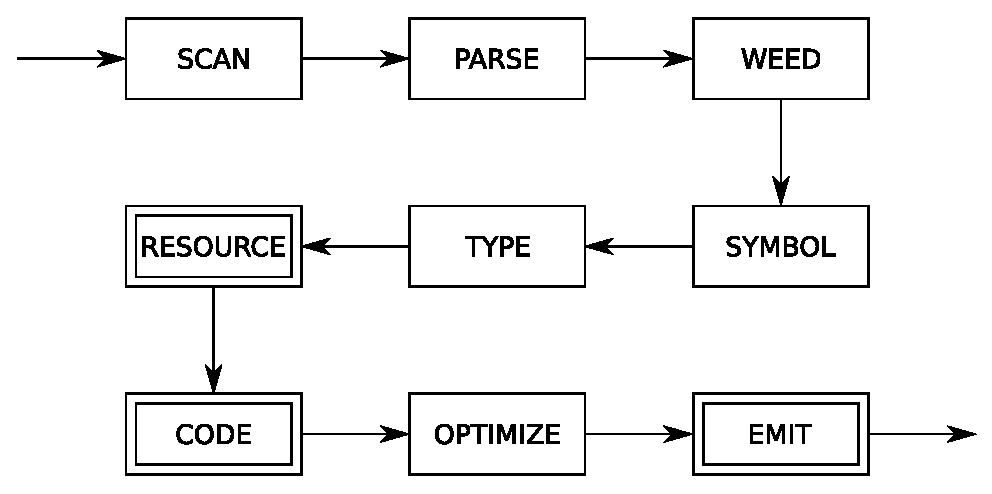
\psfig{file=figs/codegen.eps,width=20em}
\end{center}

\vfil
\end{slide*}
 
\begin{slide*}
The {\em code generation\/} phase has several sub-phases:
\begin{itemize}
\item computing {\em resources\/} such as stack layouts, offsets, labels, registers, and dimensions;
\item generating an internal representation of machine codes for statements and expressions; 
\item optimizing the code (ignored for now); and
\item emitting the code to files in assembler or binary format.
\end{itemize}
\vfil
\end{slide*}
 
\begin{slide*}
Resources in JOOS:
\begin{itemize}
\item offsets for locals and formals;
\item labels for control structures; and
\item local and stack limits for methods.
\end{itemize}
These are values that cannot be computed based on a single statement.

We must perform a global traversal of the parse trees.

\vfil
\end{slide*}
 
\begin{slide*}
Computing offsets and the locals limit:

\newcommand{\os}[1]{ \hspace*{-0.4em}\raisebox{0.2em}{\fbox{$_{#1}$}}}
\begin{scriptsize}
\begin{alltt}
public class Example \{

  public Example() \{ super(); \}

  public void Method(int p\os{1}, int q\os{2}, Example r\os{3}) \{
     int x\os{4};
     int y\os{5};
     \{ int z\os{6};
       z = 87;
     \}
     \{ boolean a\os{6};
       Example x\os{7};
       \{ boolean b\os{8};
         int z\os{9};
         b = true;
       \}
       \{ int y\os{8};
         y = x;
       \}
     \}
  \}
\}
\end{alltt}
\end{scriptsize}

The locals limit is the largest offset generated in the method + one
extra slot for {\tt this}.
\vfil
\end{slide*}
 
\begin{slide*}
Corresponding JOOS source:

\begin{scriptsize}
\begin{verbatim}

int offset, localslimit;

int nextoffset()
{ offset++;
  if (offset > localslimit) localslimit = offset;
  return offset;
}

void resFORMAL(FORMAL *f)
{ if (f!=NULL) {
     resFORMAL(f->next);
     f->offset = nextoffset();
  }
}

void resID(ID *i)
{ if (i!=NULL) {
     resID(i->next);
     i->offset = nextoffset();
  }
}

...

case blockK:
     baseoffset = offset;
     resSTATEMENT(s->val.blockS.body);
     offset = baseoffset;
     break;
\end{verbatim}
\end{scriptsize}

\vfil
\end{slide*}
 
\begin{slide*}
Computing labels for control structures:\\

\begin{tabular}{rl}
{\tt if}: & 1 label\\
{\tt ifelse}: & 2 labels\\
{\tt while}: & 2 labels\\
{\tt toString} coercion: & 2 labels\\
\verb"||" and \verb"&&": & 1 label\\
\verb"==", \verb"<", \verb">", \verb"<=", \verb">=", and \verb"!=": & 2 labels\\
\verb"!": & 2 labels
\end{tabular}
~\\
~\\

Labels are generated consecutively, for each method and constructor separately.

The Jasmin assembler converts labels to addresses. An address in Java bytecode
is a 16-bit offset with respect to the branching instruction. The target
address must be part of the code array of the same method. 
\vfil
\end{slide*}
 
\begin{slide*}
Corresponding JOOS source:

\begin{scriptsize}
\begin{verbatim}

int label;
 
int nextlabel()
{ return label++;
}

.
.
.

case whileK:
     s->val.whileS.startlabel = nextlabel();
     s->val.whileS.stoplabel = nextlabel();
     resEXP(s->val.whileS.condition);
     resSTATEMENT(s->val.whileS.body);
     break;
.
.
.

case orK:
     e->val.orE.truelabel = nextlabel();
     resEXP(e->val.orE.left);
     resEXP(e->val.orE.right);
     break;

.
.
.
\end{verbatim}
\end{scriptsize}

\vfil
\end{slide*}
 
\begin{slide*}
\begin{scriptsize}
\begin{verbatim}
typedef struct CODE {
   enum {nopCK,i2cCK,
         newCK,instanceofCK,checkcastCK,
         imulCK,inegCK,iremCK,isubCK,idivCK,iaddCK,iincCK,
         labelCK,gotoCK,ifeqCK,ifneCK,
         if_acmpeqCK,if_acmpneCK, ifnullCK,ifnonnullCK,
         if_icmpeqCK,if_icmpgtCK,if_icmpltCK,
         if_icmpleCK,if_icmpgeCK,if_icmpneCK,
         ireturnCK,areturnCK,returnCK,
         aloadCK,astoreCK,iloadCK,istoreCK,dupCK,popCK,
         swapCK,ldc_intCK,ldc_stringCK,aconst_nullCK,
         getfieldCK,putfieldCK,
         invokevirtualCK,invokenonvirtualCK} kind;
   union {
     char *newC;
     char *instanceofC;
     char *checkcastC;
     struct {int offset; int amount;} iincC;
     int labelC;
     int gotoC;
     int ifeqC;
     ...
     int istoreC;
     int ldc_intC;
     char *ldc_stringC;
     char *getfieldC;
     char *putfieldC;
     char *invokevirtualC;
     char *invokenonvirtualC;
   } val;
   struct CODE *next;
} CODE;
\end{verbatim}
\end{scriptsize}
\vfil
\end{slide*}

\begin{slide*}
Code templates:

\begin{itemize}
\item show how to generate code for each language construct;
\item ignore the surrounding context; and
\item dictate a simple, recursive strategy.
\end{itemize}
\vspace*{2ex}

Code template invariants:

\begin{itemize}
\item evaluation of a statement leaves the stack height unchanged; and
\item evaluation of an expression increases the stack height by
one.
\end{itemize}

Special case of \verb$ExpressionStatement$:
 
\begin{itemize} 
\item Expression is evaluated, result is then popped off the stack, except
\item for \verb$void$ return expressions, nothing is popped.
\end{itemize}
\vfil
\end{slide*}

\newcommand{\mm}[1]{$#1$}
 
\begin{slide*}
The statement:

\begin{scriptsize}
\begin{alltt}
    if (\mm{E}) \mm{S}
\end{alltt}
\end{scriptsize}

has code template:

\begin{scriptsize}
\begin{alltt}
    \mm{E}
    ifeq stop
    \mm{S}
    stop:
\end{alltt}
\end{scriptsize}

Corresponding JOOS source:

\begin{scriptsize}
\begin{verbatim}
case ifK:
     codeEXP(s->val.ifS.condition);
     code_ifeq(s->val.ifS.stoplabel);
     codeSTATEMENT(s->val.ifS.body);
     code_label("stop",s->val.ifS.stoplabel);
     break;
\end{verbatim}
\end{scriptsize}

\vfil
\end{slide*}
 
\begin{slide*}
The statement:
 
\begin{scriptsize}
\begin{alltt}
     if (\mm{E}) \mm{S_1} else \mm{S_2}
\end{alltt}
\end{scriptsize}
 
has code template:
 
\begin{scriptsize}
\begin{alltt}
     \mm{E}
     ifeq else
     \mm{S_1}
     goto stop
     else:
     \mm{S_2}
     stop:
\end{alltt}
\end{scriptsize}
 
Corresponding JOOS source:
 
\begin{scriptsize}
\begin{verbatim}
case ifelseK:
     codeEXP(s->val.ifelseS.condition);
     code_ifeq(s->val.ifelseS.elselabel);
     codeSTATEMENT(s->val.ifelseS.thenpart);
     code_goto(s->val.ifelseS.stoplabel);
     code_label("else",s->val.ifelseS.elselabel);
     codeSTATEMENT(s->val.ifelseS.elsepart);
     code_label("stop",s->val.ifelseS.stoplabel);
     break;
\end{verbatim}
\end{scriptsize}
\vfil
\end{slide*}

\begin{slide*}
The statement:
 
\begin{scriptsize}
\begin{alltt}
     while (\mm{E}) \mm{S}
\end{alltt}
\end{scriptsize}
 
has code template:
 
\begin{scriptsize}
\begin{alltt}
    start:
    \mm{E}
    ifeq stop
    \mm{S}
    goto start
    stop:
\end{alltt}
\end{scriptsize}
 
Corresponding JOOS source:
 
\begin{scriptsize}
\begin{verbatim}
case whileK:
     code_label("start",s->val.whileS.startlabel);
     codeEXP(s->val.whileS.condition);
     code_ifeq(s->val.whileS.stoplabel);
     codeSTATEMENT(s->val.whileS.body);
     code_goto(s->val.whileS.startlabel);
     code_label("stop",s->val.whileS.stoplabel);
     break;
\end{verbatim}
\end{scriptsize}
\vfil
\end{slide*}

\begin{slide*}
The statement:
 
\begin{scriptsize}
\begin{alltt}
     \mm{E}
\end{alltt}
\end{scriptsize}
 
has code template:
 
\begin{scriptsize}
\begin{alltt}
     \mm{E}
\end{alltt}
\end{scriptsize}

if \mm{E} has type {\tt void} and otherwise:

\begin{scriptsize}
\begin{alltt}
     \mm{E}
     pop
\end{alltt}
\end{scriptsize}
 
Corresponding JOOS source:
 
\begin{scriptsize}
\begin{verbatim}
case expK:
     codeEXP(s->val.expS);
     if (s->val.expS->type->kind!=voidK) {
        code_pop();
     }
     break;
\end{verbatim}
\end{scriptsize}
\vfil
\end{slide*}

\begin{slide*}
The local variable expression:
 
\begin{scriptsize}
\begin{alltt}
    \mm{x}
\end{alltt}
\end{scriptsize}
 
has code template:
 
\begin{scriptsize}
\begin{alltt}
    iload {\em offset(\mm{x})}
\end{alltt}
\end{scriptsize}

if \mm{x} has type {\tt int} or {\tt boolean} and otherwise:

\begin{scriptsize}
\begin{alltt}
    aload {\em offset(\mm{x})}
\end{alltt}
\end{scriptsize}
 
Corresponding JOOS source:
 
\begin{scriptsize}
\begin{verbatim}
case localSym:
  if (e->val.idE.idsym->val.localS.type->kind==refK) {
     code_aload(e->val.idE.idsym->val.localS->offset);
  } else {
     code_iload(e->val.idE.idsym->val.localS->offset);
  }      
  break;
\end{verbatim}
\end{scriptsize}

\vfil
\end{slide*}

\begin{slide*}
The assignment to a formal:
 
\begin{scriptsize}
\begin{alltt}
    \mm{x}=\mm{E}
\end{alltt}
\end{scriptsize}
 
is an expression on its own and has code template:
 
\begin{scriptsize}
\begin{alltt}
    \mm{E}
    dup
    istore {\em offset(\mm{x})}
\end{alltt}
\end{scriptsize}

if \mm{x} has type {\tt int} or {\tt boolean} and otherwise:

\begin{scriptsize}
\begin{alltt}
    \mm{E}
    dup
    astore {\em offset(\mm{x})}
\end{alltt}
\end{scriptsize}

Corresponding JOOS source:
 
\begin{scriptsize}
\begin{verbatim}
case formalSym:
     codeEXP(e->val.assignE.right);
     code_dup();
     if (e->val.assignE.leftsym->
            val.formalS->type->kind==refK) {
        code_astore(e->val.assignE.leftsym->
                       val.formalS->offset);
     } else {
        code_istore(e->val.assignE.leftsym->
                       val.formalS->offset);
     }
     break;
\end{verbatim}
\end{scriptsize}
% Note the difference of runtime return value (taken from RHS) and declared type
% of the assignment expression (taken from LHS).
\vfil
\end{slide*}

\begin{slide*}
The expression:
 
\begin{scriptsize}
\begin{alltt}
     \mm{E_1} || \mm{E_2}
\end{alltt}
\end{scriptsize}
 
has code template:
 
\begin{scriptsize}
\begin{alltt}
    \mm{E_1}
    dup
    ifne true
    pop
    \mm{E_2}
    true:
\end{alltt}
\end{scriptsize}
 
Corresponding JOOS source:
 
\begin{scriptsize}
\begin{verbatim}
case orK:
     codeEXP(e->val.orE.left);
     code_dup();
     code_ifne(e->val.orE.truelabel);
     code_pop();
     codeEXP(e->val.orE.right);
     code_label("true",e->val.orE.truelabel);
     break;
\end{verbatim}
\end{scriptsize}
\vfil
\end{slide*}

\begin{slide*}
The expression:
 
\begin{scriptsize}
\begin{alltt}
   \mm{E_1} == \mm{E_2}
\end{alltt}
\end{scriptsize}
 
has code template:
 
\begin{scriptsize}
\begin{alltt}
   \mm{E_1}
   \mm{E_2}
   if_icmpeq true
   ldc_int 0
   goto stop
   true:
   ldc_int 1
   stop:
\end{alltt}
\end{scriptsize}

if \mm{E_i} has type {\tt int} or {\tt boolean}.

Corresponding JOOS source:
 
\begin{scriptsize}
\begin{verbatim}
case eqK:
     codeEXP(e->val.eqE.left);
     codeEXP(e->val.eqE.right);
     if (e->val.eqE.left->type->kind==refK) {
       code_if_acmpeq(e->val.eqE.truelabel);
     } else {
       code_if_icmpeq(e->val.eqE.truelabel);
     }
     code_ldc_int(0);
     code_goto(e->val.eqE.stoplabel);
     code_label("true",e->val.eqE.truelabel);
     code_ldc_int(1);
     code_label("stop",e->val.eqE.stoplabel);
     break;
\end{verbatim}
\end{scriptsize}
\vfil
\end{slide*}

\begin{slide*}
The expression:
 
\begin{scriptsize}
\begin{alltt}
    \mm{E_1} + \mm{E_2}
\end{alltt}
\end{scriptsize}
 
has code template:
 
\begin{scriptsize}
\begin{alltt}
    \mm{E_1}
    \mm{E_2}
    iadd
\end{alltt}
\end{scriptsize}

if \mm{E_i} has type {\tt int} and otherwise:

\begin{scriptsize}
\begin{alltt}
    \mm{E_1}
    \mm{E_2}
    invokevirtual {\tiny\rm java/lang/String/concat(Ljava/lang/String;)
                                                   Ljava/lang/String;}
\end{alltt}
\end{scriptsize}

Corresponding JOOS source:
 
\begin{scriptsize}
\begin{verbatim}
case plusK:
     codeEXP(e->val.plusE.left);
     codeEXP(e->val.plusE.right);
     if (e->type->kind==intK) {
        code_iadd();
     } else {
        code_invokevirtual("java/lang/.../String;");
     }
     break;
\end{verbatim}
\end{scriptsize}

(A separate test of an {\tt e->tostring} field is used to handle string coercion.)

\vfil
\end{slide*}

\begin{slide*}
The expression:
 
\begin{scriptsize}
\begin{alltt}
    !\mm{E}
\end{alltt}
\end{scriptsize}
 
has code template:
 
\begin{scriptsize}
\begin{alltt}
    \mm{E}
    ifeq true
    ldc_int 0
    goto stop
    true:
    ldc_int 1
    stop:
\end{alltt}
\end{scriptsize}
 
Corresponding JOOS source:
 
\begin{scriptsize}
\begin{verbatim}
case notK:
     codeEXP(e->val.notE.not);
     code_ifeq(e->val.notE.truelabel);
     code_ldc_int(0);
     code_goto(e->val.notE.stoplabel);
     code_label("true",e->val.notE.truelabel);
     code_ldc_int(1);
     code_label("stop",e->val.notE.stoplabel);
     break;
\end{verbatim}
\end{scriptsize}
\vfil
\end{slide*}

\begin{slide*}
Alternative translation of Boolean expressions:\\
Short-circuit or Jumping code

Motivating example: Expression
\begin{center} 
\verb"!!!!!!!"\mm{E}
\end{center}
would generate lots of jumps when
using the template described earlier. (Other Boolean operations, too.)

Idea: Can encode Boolean logic by more clever introduction and swaps of
labels.

Use function {\sl trans}$(b,l,t,f)$ with:
\begin{description}
\item[$b$] Boolean expression
\item[$l$] label for evaluating current expression
\item[$t$] jump-label in case $b$ evaluates to $\mathbf{true}$ 
\item[$f$] jump-label in case $b$ evaluates to $\mathbf{false}$
\end{description}

\vfil 
\end{slide*}

\begin{slide*}
{\sl trans}(\mm{E_1} $==$ \mm{E_2},~$l$,~$t$,~$f$)=

\begin{scriptsize}
\begin{alltt}
l: \mm{E_1}
   \mm{E_2}
   if_icmpeq true
   ldc_int 0
   goto f
   true:
   ldc_int 1
   goto t
\end{alltt}
\end{scriptsize}   

\bigskip

{\sl trans}(\verb"!"\mm{E},~$l$,~$t$,~$f$)= {\sl trans}(\mm{E},~$l$,~$f$,~$t$)
   
\bigskip

{\sl trans}(\mm{E_1} \verb"&&" \mm{E_2},~$l$,~$t$,~$f$)=\\
\hspace*{5mm} {\sl trans}(\mm{E_1},~$l$,~$l'$,~$f$),
{\sl trans}(\mm{E_2},~$l'$,~$t$,~$f$)

\bigskip

{\sl trans}(\mm{E_1} \verb"||" \mm{E_2},~$l$,~$t$,~$f$)=\\
\hspace*{5mm} {\sl trans}(\mm{E_1},~$l$,~$t$,~$l'$),
{\sl trans}(\mm{E_2},~$l'$,~$t$,~$f$)

\bigskip
Jumping code can be longer in comparison but for each branch it will
usually execute less instructions.

\vfil 
\end{slide*}

\begin{slide*}
The expression:
 
\begin{scriptsize}
\begin{alltt}
     this
\end{alltt}
\end{scriptsize}
 
has code template:
 
\begin{scriptsize}
\begin{alltt}
     aload 0
\end{alltt}
\end{scriptsize}
 
Corresponding JOOS source:
 
\begin{scriptsize}
\begin{verbatim}
case thisK:
     code_aload(0);
     break;
\end{verbatim}
\end{scriptsize}
\vfil
\end{slide*}

\begin{slide*}
The expression:
 
\begin{scriptsize}
\begin{alltt}
    null
\end{alltt}
\end{scriptsize}
 
has code template:
 
\begin{scriptsize}
\begin{alltt}
    ldc_string "null"
\end{alltt}
\end{scriptsize}

if it is {\tt toString} coerced and otherwise:

\begin{scriptsize}
\begin{alltt}
    aconst_null
\end{alltt}
\end{scriptsize}

Corresponding JOOS source:
 
\begin{scriptsize}
\begin{verbatim}
case nullK:
     if (e->tostring) {
        code_ldc_string("null");
     } else {
        code_aconst_null();
     }
     break;
\end{verbatim}
\end{scriptsize}

\vfil
\end{slide*}
 
\begin{slide*}
The expression:

\begin{scriptsize}
\begin{alltt}
    \mm{E}.\mm{m}(\mm{E_1},\ldots,\mm{E_n})
\end{alltt}
\end{scriptsize}
 
has code template:
 
\begin{scriptsize}
\begin{alltt}
    \mm{E}
    \mm{E_1}
    .
    .
    .
    \mm{E_n}
    invokevirtual {\em signature(class(\mm{E}),\mm{m})}

\end{alltt}
\end{scriptsize}

{\tt\em class(\mm{E})} is the declared class of \mm{E}.

{\tt\em signature(C,\mm{m})} is the signature of the first implementation
of \mm{m} that is found from {\tt\em C}.
\vfil
\end{slide*}

\begin{slide*}
The expression:
 
\begin{scriptsize}
\begin{alltt}
    super.\mm{m}(\mm{E_1},\ldots,\mm{E_n})
\end{alltt}
\end{scriptsize}
 
has code template:
 
\begin{scriptsize}
\begin{alltt}
    aload 0
    \mm{E_1}
    .
    .
    .
    \mm{E_n}
    invokespecial {\em signature(parent(thisclass)),\mm{m})}

\end{alltt}
\end{scriptsize}

{\tt\em thisclass} is the current class.
 
{\tt\em parent(C)} is the parent of {\tt\em C} in the hierarchy.
 
{\tt\em signature(C,\mm{m})} is the signature of the first implementation
of \mm{m} that is found from {\tt\em parent(C)}.
\vfil
\end{slide*}

\begin{slide*}
Corresponding JOOS source:
 
\begin{scriptsize}
\begin{verbatim}

case invokeK:
     codeRECEIVER(e->val.invokeE.receiver);
     codeARGUMENT(e->val.invokeE.args);
     switch (e->val.invokeE.receiver->kind) {
       case objectK:
             { SYMBOL *s;
                s = lookupHierarchyClass(
                          e->val.invokeE.method->name,
                          e->val.invokeE.receiver->
                             objectR->type->class);
                code_invokevirtual(
                     codeMethod(s,e->val.invokeE.method)
                );
              }
            break;
       case superK:
            { CLASS *c;
              c = lookupHierarchyClass(
                        e->val.invokeE.method->name,
                        currentclass->parent);
              code_invokenonvirtual(
                   codeMethod(c,e->val.invokeE.method)
              );
            }
            break;
     }
     break;
\end{verbatim}
\end{scriptsize}

\vfil
\end{slide*}
 
\begin{slide*}
A {\tt toString} coercion of the expression:

\begin{scriptsize}
\begin{alltt}
    \mm{E}
\end{alltt}
\end{scriptsize}

has code template:

\newcommand{\II}{$\mathrm{\langle}$init$\mathrm{\rangle}$}
\begin{scriptsize}
\begin{alltt}
    new {\tiny\rm java/lang/Integer}
    dup
    \mm{E}
    invokespecial {\tiny\rm java/lang/Integer/\II{}(I)V}
    invokevirtual {\tiny\rm java/lang/Integer/toString()Ljava/lang/String;}
\end{alltt}
\end{scriptsize}

if \mm{E} has type {\tt int}, and:

\begin{scriptsize}
\begin{alltt}
    new {\tiny\rm java/lang/Boolean}
    dup
    \mm{E}
    invokespecial {\tiny\rm java/lang/Boolean/\II{}(Z)V}
    invokevirtual {\tiny\rm java/lang/Boolean/toString()Ljava/lang/String;}
\end{alltt}
\end{scriptsize}
 
if \mm{E} has type {\tt boolean}, and:

\begin{scriptsize}
\begin{alltt}
    new {\tiny\rm java/lang/Character}
    dup
    \mm{E}
    invokespecial {\tiny\rm java/lang/Character/\II{}(C)V}
    invokevirtual {\tiny\rm java/lang/Character/toString()Ljava/lang/String;}
\end{alltt}
\end{scriptsize}

if \mm{E} has type {\tt char}.

\vfil
\end{slide*}
 
\begin{slide*}
A {\tt toString} coercion of the expression:
 
\begin{scriptsize}
\begin{alltt}
    \mm{E}
\end{alltt}
\end{scriptsize}
 
has code template:

\begin{scriptsize}
\begin{alltt}
    \mm{E}
    dup
    ifnull nulllabel
    invokevirtual {\em signature(class(\mm{E}),{\rm toString})}
    goto stoplabel
    nulllabel:
    pop
    ldc_string "null"
    stoplabel:
\end{alltt}
\end{scriptsize}

if \mm{E} does not have type {\tt int}, {\tt boolean}, or {\tt char}.
\vfil
\end{slide*}

\begin{slide*}
Computing the stack limit:

\begin{scriptsize}
\begin{verbatim}
public void Method() {
  int x, y;
  x = 12; y = 87;
  x:=2*(x+y*(x-y));
}
\end{verbatim}
\end{scriptsize}

\newcommand{\LA}{$\leftarrow$}
\newcommand{\zap}{\hspace*{-0.415em}}
\begin{scriptsize}
\begin{alltt}
.method public Method()V
  .limit locals 3
  .limit stack 5
  ldc 12       \LA{} 1
  dup          \LA{} 2
  istore_1     \LA{} 1
  pop          \LA{} 0
  ldc 87       \LA{} 1
  dup          \LA{} 2
  istore_2     \LA{} 1
  pop          \LA{} 0
  iconst_2     \LA{} 1
  iload_1      \LA{} 2
  iload_2      \LA{} 3
  iload_1      \LA{} 4
  iload_2      \LA{} \zap{}\fbox{5}
  isub         \LA{} 4
  imul         \LA{} 3
  iadd         \LA{} 2
  imul         \LA{} 1
  dup          \LA{} 2
  istore_1     \LA{} 1
  pop          \LA{} 0
  return
.end method
\end{alltt}
\end{scriptsize}
\vfil
\end{slide*}

\begin{slide*}
The stack limit 
is the maximum height of the stack during the evaluation of an expression 
in the method.\\

This requires detailed knowledge of:
\begin{itemize}
\item the code that is generated; and
\item the virtual machine.
\end{itemize}
\vspace*{2ex}

Stupid \raisebox{-0.5ex}{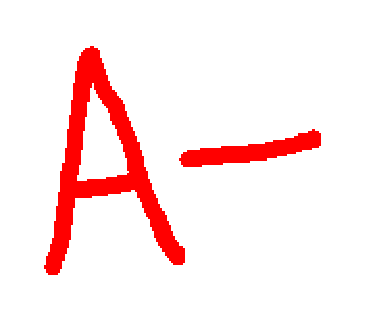
\epsfig{file=grade.eps,width=2em}} JOOS source:
\begin{verbatim}
int limitCODE(CODE *c)
{ return 25;
}
\end{verbatim}

\vfil
\end{slide*}

\begin{slide*}
Code is emitted in Jasmin format:

\newcommand{\VV}{$\vdots$}
\begin{scriptsize}
\begin{alltt}

    .class public \mm{C}
    .super{\em parent(\mm{C})}
    
    .field protected \mm{x_1}{\em type(\mm{x_1})}
    \VV{}
    .field protected \mm{x_k}{\em type(\mm{x_k})}

    .method public \mm{m_1}{\em signature(\mm{C},\mm{m_1})}
       .limit locals \mm{l_1}
       .limit stack \mm{s_1}
       \mm{S_1}
    .end method

    \VV{}

    .method public \mm{m_n}{\em signature(\mm{C},\mm{m_n})}
       .limit locals \mm{l_n}
       .limit stack \mm{s_n}
       \mm{S_n}
    .end method
\end{alltt}
\end{scriptsize}

\vfil
\end{slide*}

\begin{slide*}
The signature of a method {\tt m} in a class {\tt C} with
argument types $\tau_1,\ldots,\tau_k$ and return type $\tau$
is represented in Jasmin as:
\begin{center}
{\tt C/m(}{\em {\small rep}($\tau_1$)\ldots {\small rep}($\tau_k$)}{\tt )}{\small rep}($\tau$) 
\end{center}
where:
\begin{itemize}
\item {\em {\small rep}({\tt int}) = {\tt I}}
\item {\em {\small rep}({\tt boolean}) = {\tt Z}}
\item {\em {\small rep}({\tt char}) = {\tt C}}
\item {\em {\small rep}({\tt void}) = {\tt V}}
\item {\em {\small rep}({\tt C}) = {\tt LC;}}
\end{itemize}
\vfil
\end{slide*}
 
\begin{slide*}
A tiny JOOS class:

\begin{scriptsize}
\begin{verbatim}

import joos.lib.*;
 
public class Tree {
  protected Object value;
  protected Tree left;
  protected Tree right;
 
  public Tree(Object v, Tree l, Tree r)
    { super();
      value = v;
      left = l; 
      right = r;
    }
 
  public void setValue(Object newValue)
    { value = newValue; }
}
\end{verbatim}
\end{scriptsize}

\vfil
\end{slide*}
 
\begin{slide*}
The compiled Jasmin file:

\begin{scriptsize}
\begin{verbatim}
.class public Tree
.super java/lang/Object
.field protected value Ljava/lang/Object;
.field protected left LTree;
.field protected right LTree;
 
.method public <init>(Ljava/lang/Object;LTree;LTree;)V
  .limit locals 4
  .limit stack 3
  aload_0
  invokenonvirtual java/lang/Object/<init>()V
  aload_0
  aload_1
  putfield Tree/value Ljava/lang/Object;
  aload_0
  aload_2
  putfield Tree/left LTree;
  aload_0
  aload_3
  putfield Tree/right LTree;
  return
.end method
 
.method public setValue(Ljava/lang/Object;)V
  .limit locals 2
  .limit stack 3
  aload_0
  aload_1
  putfield Tree/value Ljava/lang/Object;
  return
.end method
\end{verbatim}
\end{scriptsize}

\vfil
\end{slide*}
 
\begin{slide*}
Hex dump of the class file:

\begin{scriptsize}
\begin{verbatim}

cafe babe 0003 002d 001a 0100 064c 5472
6565 3b07 0010 0900 0200 0501 0015 284c
6a61 7661 2f6c 616e 672f 4f62 6a65 6374
3b29 560c 0018 0001 0100 0654 7265 652e
6a01 000a 536f 7572 6365 4669 6c65 0100
0443 6f64 6507 000d 0c00 0e00 1209 0002
0017 0100 2128 4c6a 6176 612f 6c61 6e67
2f4f 626a 6563 743b 4c54 7265 653b 4c54
7265 653b 2956 0100 106a 6176 612f 6c61
6e67 2f4f 626a 6563 7401 0005 7661 6c75
650c 0011 0019 0100 0454 7265 6501 0006
3c69 6e69 743e 0100 124c 6a61 7661 2f6c
616e 672f 4f62 6a65 6374 3b0a 0009 000f
0100 0873 6574 5661 6c75 6509 0002 000a
0100 046c 6566 740c 0016 0001 0100 0572
6967 6874 0100 0328 2956 0021 0002 0009
0000 0003 0006 000e 0012 0000 0006 0016
0001 0000 0006 0018 0001 0000 0002 0001
0011 000c 0001 0008 0000 0020 0003 0004
0000 0014 2ab7 0013 2a2b b500 152a 2cb5
000b 2a2d b500 03b1 0000 0000 0001 0014
0004 0001 0008 0000 0012 0003 0002 0000
0006 2a2b b500 15b1 0000 0000 0001 0007
0000 0002 0006
\end{verbatim}
\end{scriptsize}

\vfil
\end{slide*}
 
\begin{slide*}
The testing strategy for the code generator involves 
two phases.\\

First a careful
argumentation that each code template is correct.\\

Second a demonstration that each code template is generated correctly.\\

\vfil
\end{slide*}
 
\begin{slide*}
\vfil
\end{slide*}
 
\begin{slide*}
\vfil
\end{slide*}
 
\begin{slide*}
\vfil
\end{slide*}
 
\begin{slide*}
\vfil
\end{slide*}
 
\begin{slide*}
\vfil
\end{slide*}
 
\begin{slide*}
\vfil
\end{slide*}
 
\begin{slide*}
\vfil
\end{slide*}
 
\end{document}

